\section*{Utregning av virkningsgrader}
\setcounter{section}{5}
\addcontentsline{toc}{section}{Utregning av virkningsgrader}

\setcounter{subsection}{0}


\subsection{Utregning av virkningsgrader}
Turtall, dreiemoment, volumstrøm og trykk ble direkte avlest fra lab-oppsettet under forsøket. Basert på disse målte verdiene ble mekanisk effekt, hydraulisk effekt og virkningsgrad beregnet. Pelton-turbinen ble kjørt med en vannstrøm på omtrent 115 $L/min$ (0,00192 $m^3/s$) og 170 $L/min$ (0,00283 $m^3/s$), samt et turtall på om lag 2900 rpm.
Resultatene for nålposisjon 3 er presentert i tabell \ref{tab:pelton}, mens resultatene for nålposisjon 7 er presentert i tabell \ref{tab:pelton2}.

\begin{table}[htbp]
\centering
\caption{Måledata og beregnede verdier for Pelton-turbin. Nålposisjon 3.}
\label{tab:pelton}
\small
\begin{tabular}{
  c
  S[table-format=4.0]
  S[table-format=2.2]
  S[table-format=2.2]
  S[table-format=1.2]
  S[table-format=6.0]
  S[table-format=1.5]
  S[table-format=3.2]
  S[table-format=3.2]
  S[table-format=2.2]
}
\toprule
{\textbf{Måling}} &
{\textbf{$n_{pumpe}$}} &
{\textbf{$n_{pumpe}$}} &
{\textbf{$n_{turbin}$}} &
{\textbf{$M$}} &
{\textbf{$p_3$}} &
{\textbf{$Q$}} &
{\textbf{$P_{hyd}$}} &
{\textbf{$P_{mech}$}} &
{\textbf{$\eta$}} \\
 &
{\small [1/min]} &
{\small [1/s]} &
{\small [1/s]} &
{\small [Nm]} &
{\small [Pa]} &
{\small [m$^3$/s]} &
{\small [W]} &
{\small [W]} &
{\small [\%]} \\
\midrule
1 & 2909 & 48,48 & 24,53 & 0,75 & 314000 & 0,00192 & 413,49 & 115,61 & 27,96 \\
2 & 2909 & 48,48 & 21,87 & 1,34 & 314000 & 0,00192 & 413,49 & 184,11 & 44,52 \\
3 & 2909 & 48,48 & 17,55 & 2,06 & 314000 & 0,00192 & 413,49 & 227,16 & 54,94 \\
4 & 2909 & 48,48 & 14,78 & 2,60 & 314000 & 0,00192 & 413,49 & 241,50 & 58,41 \\
5 & 2909 & 48,48 &  9,67 & 3,30 & 314000 & 0,00192 & 413,49 & 200,43 & 48,47 \\
6 & 2909 & 48,48 &  2,83 & 4,00 & 314000 & 0,00192 & 413,49 &  71,21 & 17,22 \\
7 & 2909 & 48,48 &  0,00 & 4,60 & 314000 & 0,00192 & 413,49 &   0,00 &  0,00 \\
\bottomrule
\end{tabular}
\end{table}

%%%%%%%%%%%%%%%%%% Tabell 2 %%%%%%%%%%%%%%%%%%%%%%%%%

\begin{table}[htbp]
\centering
\caption{Måledata og beregnede verdier for Pelton-turbin. Nålposisjon 7.}
\label{tab:pelton2}
\small
\begin{tabular}{
  c
  S[table-format=4.0]
  S[table-format=2.2]
  S[table-format=2.2]
  S[table-format=1.2]
  S[table-format=6.0]
  S[table-format=1.5]
  S[table-format=3.2]
  S[table-format=3.2]
  S[table-format=2.2]
}
\toprule
{\textbf{Måling}} &
{\textbf{$n_{pumpe}$}} &
{\textbf{$n_{pumpe}$}} &
{\textbf{$n_{turbin}$}} &
{\textbf{$M$}} &
{\textbf{$p_3$}} &
{\textbf{$Q$}} &
{\textbf{$P_{hyd}$}} &
{\textbf{$P_{mech}$}} &
{\textbf{$\eta$}} \\
 &
{\small [1/min]} &
{\small [1/s]} &
{\small [1/s]} &
{\small [Nm]} &
{\small [Pa]} &
{\small [m$^3$/s]} &
{\small [W]} &
{\small [W]} &
{\small [\%]} \\
\midrule
1 & 2899 & 48,32 & 22,03 & 0,75 & 263000 & 0,00283 & 472,57 & 103,83 & 21,97 \\
2 & 2899 & 48,32 & 20,07 & 1,34 & 263000 & 0,00283 & 472,57 & 168,95 & 35,75 \\
3 & 2899 & 48,32 & 17,00 & 2,06 & 263000 & 0,00283 & 472,57 & 220,04 & 46,56 \\
4 & 2899 & 48,32 & 14,67 & 2,60 & 263000 & 0,00283 & 472,57 & 239,60 & 50,70 \\
5 & 2899 & 48,32 & 11,50 & 3,30 & 263000 & 0,00283 & 472,57 & 238,45 & 50,46 \\
6 & 2899 & 48,32 &  7,83 & 4,00 & 263000 & 0,00283 & 472,57 & 196,87 & 41,66 \\
7 & 2899 & 48,32 &  3,33 & 4,60 & 263000 & 0,00283 & 472,57 &  96,34 & 20,39 \\
8 & 2899 & 48,32 &  0,00 & 5,30 & 263000 & 0,00283 & 472,57 &   0,00 &  0,00 \\
\bottomrule
\end{tabular}
\end{table}



%%%%%%%%%%%%%%%%%%% Graf %%%%%%%%%%%%%%%%%%%%%%%%%%

\begin{figure}[H]
\centering
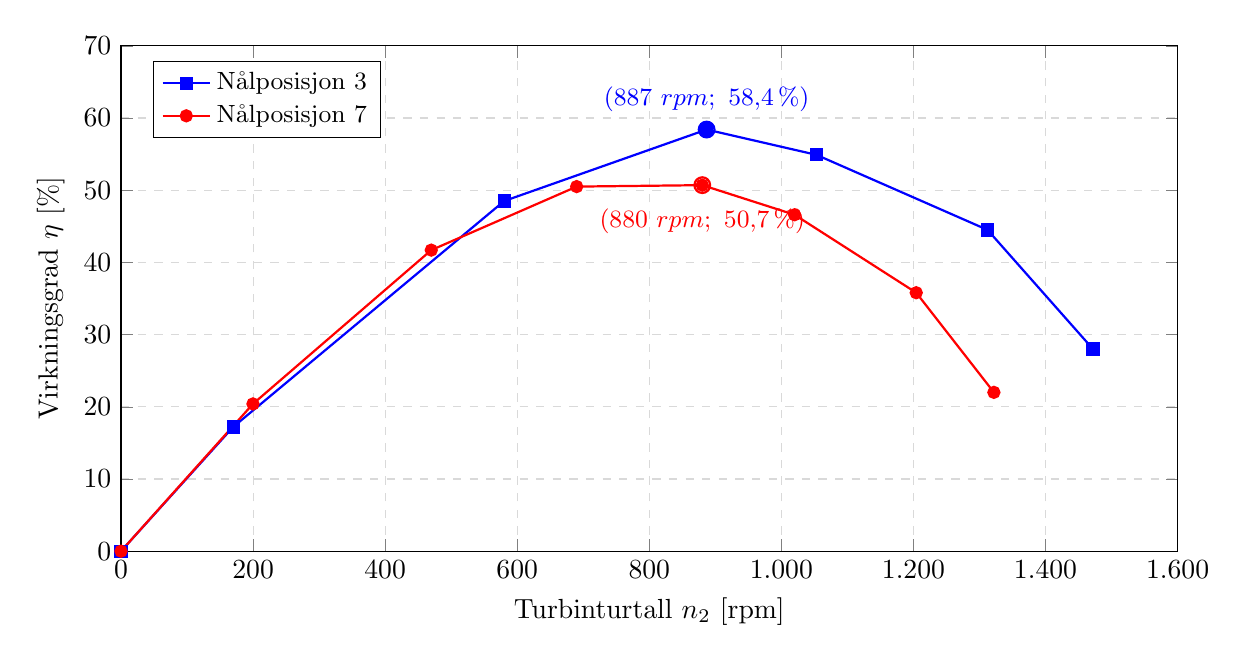
\begin{tikzpicture}
\begin{axis}[
    width=15cm,
    height=8cm,
    xlabel={Turbinturtall $n_2$ [rpm]},
    ylabel={Virkningsgrad $\eta$ [\%]},
    xmin=0, xmax=1600,
    ymin=0, ymax=70,
    grid=major,
    grid style={dashed, gray!30},
    legend pos=north west,
    legend style={font=\small},
    tick label style={/pgf/number format/use comma},
    every axis plot/.append style={thick},
]

\addplot[color=blue, mark=square*, mark size=2pt] coordinates {
    (0,  0.0)
    (169.8, 17.2)
    (580.2, 48.5)
    (886.8, 58.4)
    (1053.0, 54.9)
    (1312.2, 44.5)
    (1471.8, 28.0)
};
\addlegendentry{Nålposisjon 3}

\addplot[color=red, mark=*, mark size=2pt] coordinates {
    (0,  0.0)
    (199.8, 20.4)
    (469.8, 41.7)
    (690.0, 50.5)
    (880.2, 50.7)
    (1020.0, 46.6)
    (1204.2, 35.8)
    (1321.8, 22.0)
};
\addlegendentry{Nålposisjon 7}

% Toppunkt nålposisjon 3
\node[circle, draw=blue, inner sep=2pt, thick] at (axis cs:886.8, 58.4) {};
\node[anchor=south, blue, font=\small]
    at (axis cs:886.8, 59.5) {$(887\ \text{rpm};\ 58{,}4\,\%)$};

% Toppunkt nålposisjon 7
\node[circle, draw=red, inner sep=2pt, thick] at (axis cs:880.2, 50.7) {};
\node[anchor=north, red, font=\small]
    at (axis cs:880.2, 48.8) {$(880\ \text{rpm};\ 50{,}7\,\%)$};

\end{axis}
\end{tikzpicture}
\caption{Virkningsgrad som funksjon av turbinturtall for to nålposisjoner. Toppunktene er markert.}
\label{fig:virkningsgrad}
\end{figure}

\subsection{Diskusjon}
Maksimal virkningsgrad for nålposisjon 3 ble målt til 58,4\% ved et turtall på 14,78 omdreininger per sekund (887 rpm), mens nålposisjon 7 oppnådde en maksimal virkningsgrad på 50,7\% ved 14,67 omdreininger per sekund (880 rpm). Av de to nålposisjonene, presterte nålposisjon 3 bedre i henhold til maksimal utnyttelse av virkningsgrad.

At nålposisjon 3 gir høyere maksimal virkningsgrad enn nålposisjon 7, tyder på at den lavere vannføringen ved nålposisjon 3 ga et mer gunstig driftspunkt for turbinen. Ved nålposisjon 7 er dyseåpningen større, og volumstrømmen blir høyere. Dette gir større hydraulisk effekt inn i systemet, men resultatene viser at turbinen ikke klarte å omdanne denne ekstra tilførte effekten like effektivt til mekanisk effekt på akselen. Mulige årsaker er større strømnings- og spruttap, mindre optimal treffvinkel mot skovlene eller økte tap i bremsesystemet ved høyere vannføring.

De målte virkningsgradene fremstår rimelige for et lite laboratorieoppsett, men de er lavere enn det som normalt forventes for større, optimaliserte Pelton-turbiner i fullskala drift.

For begge nålposisjonene øker virkningsgraden først når belastningen på turbinen økes. Ved lav belastning er dreiemomentet lavt, og den mekaniske effekten på akselen blir derfor liten selv om turtallet er høyt. Når belastningen økes, øker dreiemomentet, og turbinen klarer å hente ut en større del av den hydrauliske effekten fra vannstrålen. Etter et visst punkt faller virkningsgraden igjen fordi belastningen blir så høy at turtallet reduseres betydelig. Da reduseres den mekaniske effekten, selv om dreiemomentet fortsatt er høyt. Dette forklarer hvorfor virkningsgraden får et tydelig maksimum.

Det ble ikke gjennomført målinger for alle tilgjengelige nålposisjoner, så vi kan ikke fastslå hvilken innstilling som gir best resultat totalt sett.

\subsection{Usikkerhetsvurdering}

Resultatene må vurderes med noe usikkerhet. Momentmålingen var sensitiv og kunne variere før systemet stabiliserte seg. Små avlesningsfeil i dreiemoment og turtall får direkte betydning for beregnet mekanisk effekt. I tillegg ble bare to nålposisjoner undersøkt, slik at forsøket ikke kan fastslå hvilken innstilling som faktisk gir høyest virkningsgrad. Resultatene viser derfor bare hvilken av de to undersøkte innstillingene som ga best ytelse.
